\documentclass[10pt]{beamer}

\usetheme{metropolis}
\usepackage{appendixnumberbeamer}
\usepackage{graphicx}
\usepackage{booktabs}
\usepackage[scale=2]{ccicons}
\usepackage{biblatex}
\usepackage{pgfplots}
\usepgfplotslibrary{dateplot}
\addbibresource{GeneticAlgorithms.bib}
\usepackage{xspace}
\usepackage{caption}
\newcommand{\themename}{\textbf{\textsc{metropolis}}\xspace}


\title{Finding Many Stable Molecular Arrangements}
\subtitle{Conformational Searching with Genetic Algorithms}
\date{\today}
\author{Evan Curtin}
\institute{University of Illinois at Urbana-Champaign}

\begin{document}

\maketitle

\begin{frame}{Outline}
  \setbeamertemplate{section in toc}[sections numbered]
  \tableofcontents[hideallsubsections]
\end{frame}

\section{Background Information}

\begin{frame}[fragile]{The Problem}
	\begin{itemize}[<+->]
		\item[] {Computational methods require knowledge of molecular structure}
		\begin{itemize}
			\item[$\Rightarrow$] {We need to find the lowest energy structure}
		\end{itemize}
		\item[] {The potential energy surface (PES) is high dimensional and has many minima}
		\begin{itemize}
			\item[$\Rightarrow$] {We can't tell for sure if we've found the \alert{\textbf{global}} minimum}
		\end{itemize}
		\item[] {We may need information about one or more low-energy conformations}
		\begin{itemize}
			\item[$\Rightarrow$] {Ok, let's find them all!}
		\end{itemize}	
	\end{itemize}
\end{frame}

{%
\setbeamertemplate{frame footer}{Supady, A.; Blum, V.; Baldauf, C. J. Chem. Inf. Model. 2015, 55 (11), 2338–2348.}
\begin{frame}[fragile]{Possible Solutions}
	\begin{itemize}[<+->]
		\item[] {Many techniques are well established}
		\item[] {None are perfect}
	\end{itemize}
	\begin{figure}
		\includegraphics[width=\linewidth]{images/ImplementationTables.PNG}
	\end{figure}
\end{frame}
}

\begin{frame}{Desirables}
	\begin{itemize}[<+->]
		\item Accurate energies \& Structures, \emph{ab initio} or DFT
		\item {Minimize number of geometry optimizations}
		\item {Find the entire low energy population of conformations}
		\item {Minimal human input}
		\item {Parallel-Scalable}
	\end{itemize}	
\end{frame}

\section{The Genetic Algorithm}

{%
	\setbeamertemplate{frame footer}{Carwright, H. Reviews in Computational Chemistry 2007 (25), pp 349–389.}
\begin{frame}{Outline}
	\begin{columns}[c] % align columns
		\begin{column}{.48\textwidth}
			\begin{itemize}
				\item {Inspired by biological evolution}
				\item {Evolve a population over generations}
				\item {Survival of the fittest}
				\item {Requirements:}
				\begin{itemize}
					\item {Represent individuals as vector}
					\item {Fitness function}
				\end{itemize}
				\item{$v = \left(\begin{smallmatrix}
					x_1 & y_1 & z_1 & x_2 &  y_2 & z_2 &
					... & x_N & y_N & z_N
					\end{smallmatrix}\right)$}
				\item{$F = \frac{E_{max} - E}{E_{max} - E_{min}}$}
			\end{itemize}

		\end{column}
		\hfill
		\begin{column}{0.48\textwidth}
			\begin{figure}
			\includegraphics[width=0.8\linewidth]{images/GA_outline_Carwright.PNG}
			\end{figure}
		\end{column}	
	\end{columns}
\end{frame}
}

\begin{frame}{Selecting Parents}
	\begin{columns}[c] % align columns
		\begin{column}{.48\textwidth}
			\begin{itemize}
				\item {Several methods are common}
				\item {Reinforce good characteristics}
				\item {Still give losers a chance}
				\item {'Breed' pairs of winners}
			\end{itemize}				
		\end{column}
		\hfill
		\begin{column}{0.48\textwidth}
		    \begin{overprint}
				\onslide<1>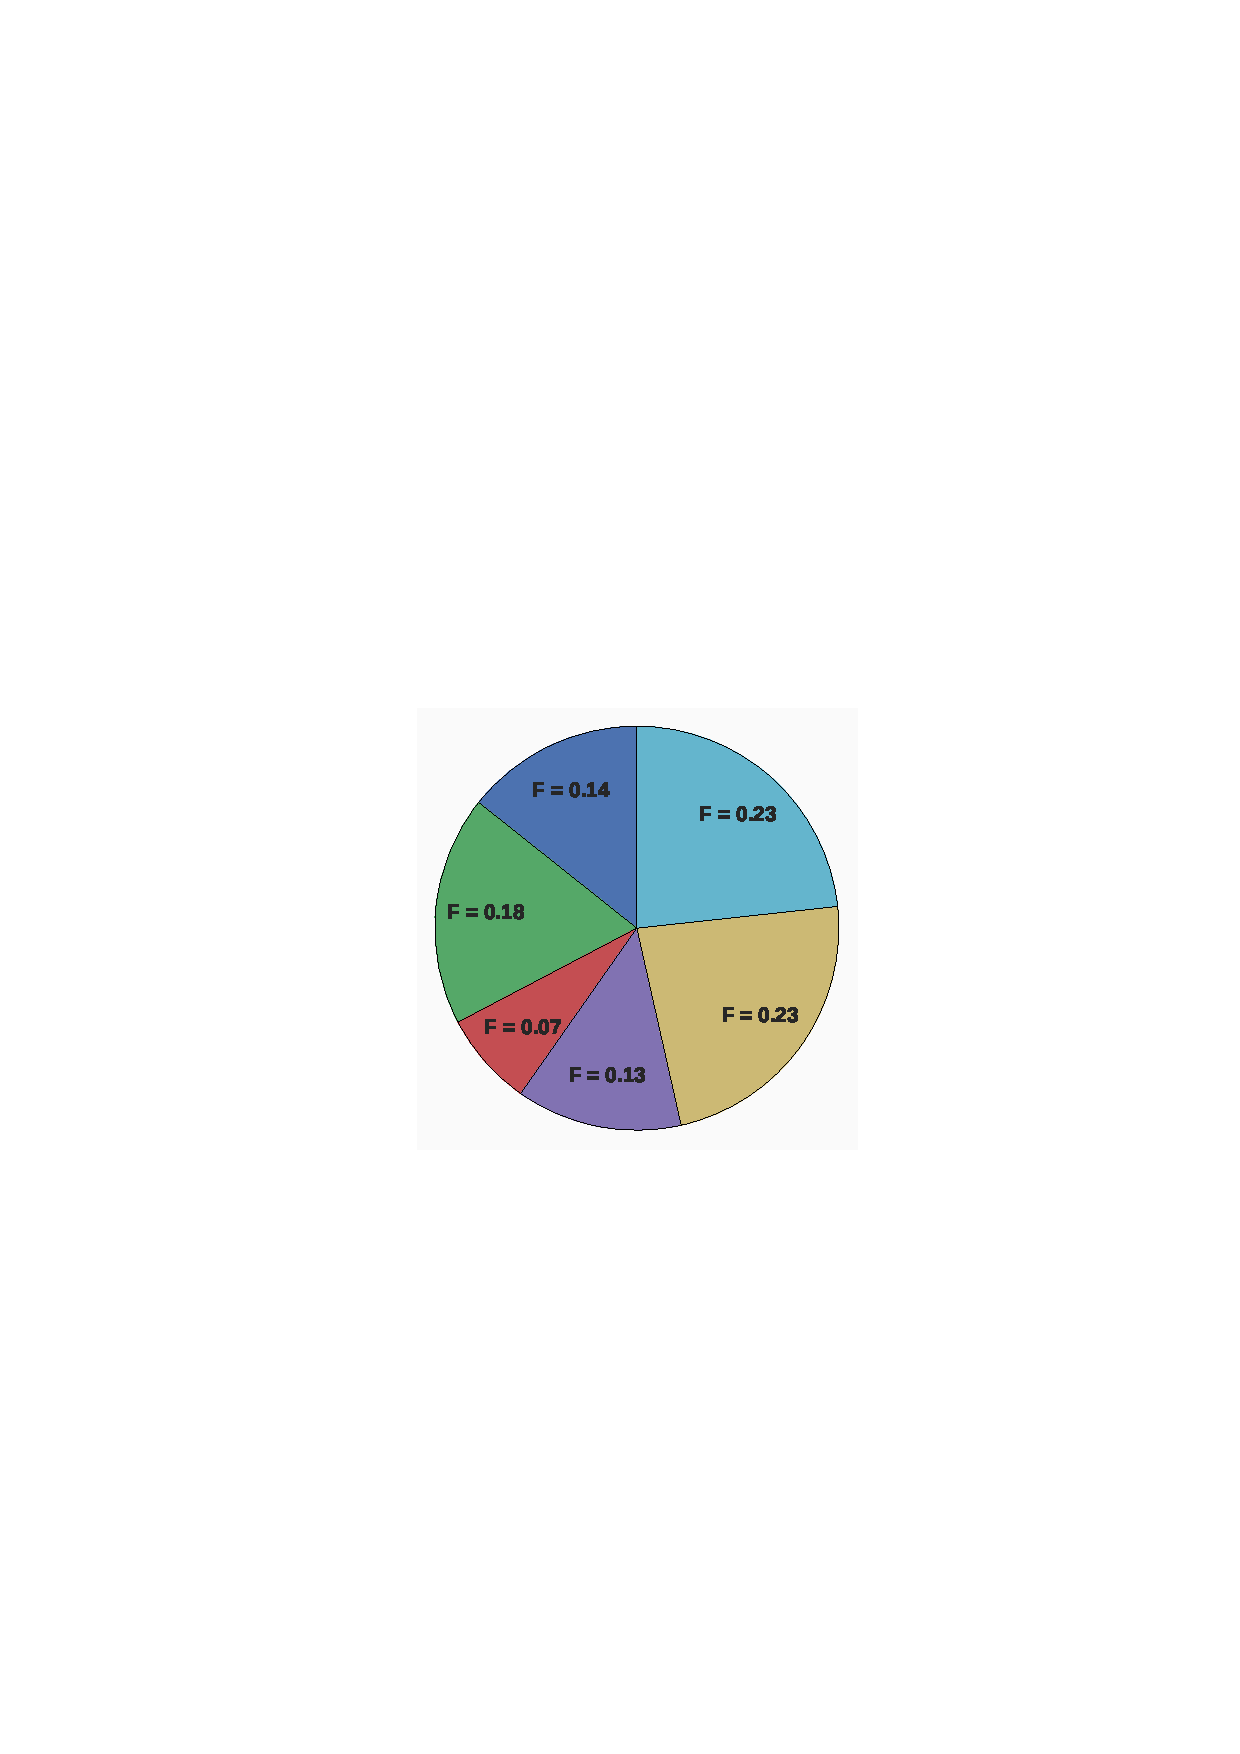
\includegraphics[width=\linewidth]{images/pie1.png}
				\onslide<2>\includegraphics[width=\linewidth]{images/pie2.png}
			\end{overprint}
		\end{column}	
	\end{columns}
\end{frame}

{%
\setbeamertemplate{frame footer}{http://www.turingfinance.com/computational-finance
	
-updates-ieee-world-congress-computational-intelligence}
\begin{frame}{The Next Generation}
	\begin{itemize}[<+->]
		\item[]{
		\begin{figure}
			\includegraphics[width=0.9\linewidth]{images/Genes_turingFinance.png}
		\end{figure}}
		\item[]{~\\Crossover distinguishes this from Monte Carlo}
	\end{itemize}
\end{frame}
}

\section{Conclusion}

\begin{frame}[standout]
  Questions?
\end{frame}

\appendix

\begin{frame}[fragile]{Backup slides}
a
\end{frame}

\end{document}
